% this template is adapted for PDF LaTeX
\documentclass[conference]{IEEEtran}

\usepackage[pdftex]{graphicx}
\usepackage[T1]{fontenc}
\usepackage{gensymb}
\usepackage{float}
\usepackage{comment}
 
% correct bad hyphenation here
%\hyphenation{op-tical net-works semi-conduc-tor}

\usepackage[swedish]{babel}
\usepackage{url}

\title{Ljusets Diffraktion}

\author{\IEEEauthorblockN{Lundberg, R. Lundell, J. Sjöholm, H.\\}
\IEEEauthorblockA{Lunds Tekniska Högskola\\
Lund, Sverige\\
Email: \{richard@fiskgjuse.com, jacoblundell@hotmail.se, hampus.sjoholm@gmail.com\}}
\and
\IEEEauthorblockN{Eric Nilsson\\}
\IEEEauthorblockA{Lunds Tekniska Högskola\\
	Lund, Sverige\\}}

%----------------------------------------------------------------

\begin{document}
\maketitle

\begin{abstract}
I rapportens första del undersöktes de diffraktionsmönster som uppstår då laserljus går genom olika typer av öppningar. Resultatet visade att flera aspekter hos diffraktionsmönstret, som i vilket eller vilka ledder det bildas i och dess utseende, beror på öppningens form och storlek. I den andra delen undersöktes spektrallinjerna från ljuset av ett grundämne. Grundämnet kunde fastställas till kadmium. I den tredje delen bestämdes fyra gitters egenskaper - antal spalter och skillnaden mellan gitternas spaltbredd - utifrån det diffraktionsmönster som uppstår då laserljus går genom dem. Resultatet visade att de alla hade samma spaltbredd och 1, 2, 3 respektive 4 spalter. Därtill bestämdes en grön lasers våglängd med samma metod. Resultatet visade att lasern har våglängden 520 nm.    \end{abstract}

%------------------------------------------------------------------------- 

\section{Introduktion}
Rapporten går ut på att studera fenomenen \emph{interferens} och \emph{diffraktion} av ljus. Specifikt  \emph{Fraunhofer-} och \emph{Fresnelböjning} som uppstår då  parallella respektive icke-parallella ljusstrålar träffar en spalt. Samt att studera ljus genom en kollimatorspalt kombinerat med en spektrallampa för att göra en primitiv typ av våglängdsbestämning av ett ljusspektrum. Utefter våglängdsbestämningen för varje individuell spektrallinje kan mätningar jämföras med ett register av mätningar för olika grundämnen. På så vis kan atomslaget i en spektrallampa identifieras. 

%-------------------------------------------------------------------------

\section{Teori}
Allmänt: \\
$ \lambda $ = Våglängd(i nanometer)

\subsection{Diffraktionsexperiment med laserljus}
Vågor som passerar genom en öppning böjs enligt \emph{Huygens princip} som säger att varje punkt på en vågfront är en källa för cirkulära elementarvågor. \cite{Fraunhofer} säger att \textbf{Fraunhoferböjning} uppstår då parallella ljusstrålar träffar en spalt. Följande formler presenterar de punkter där det uppstår destruktiv interferens mellan ljusstrålar som böjs genom en öppning (\emph{Böjningsminimum}).
 \vspace{12pt}

\textbf{Böjningsmin för en spalt: \\}
\begin{math} 
\emph{b}\sin(\theta) = m\lambda
\end{math}\\
där $ m = \pm{1}, \pm{2}, \pm{3},...$ och \emph{b} är spaltbredden. $\lambda$ är våglängden och $\theta$ är vinkeln mellan centralmax. och böjningsmin. m.
\vspace{12pt}

\textbf{Böjningsmin för en rund öppning: \\}
\begin{math}
\emph{D}\sin(\theta) = k\lambda\\
\end{math}
där $ k = \pm{1, 22}; \pm{2, 23}; \pm{3, 24}; \pm{4, 25}; \pm{5, 25}; ...\\
$ och D är diametern hos öppningen, $\lambda$ är våglängden och $\theta$ är vinkeln mellan centralmax. och böjningsmin. k.
 \vspace{12pt}

Enligt \cite{Fraunhofer} uppstår \textbf{Fresnelböjning} då icke-paralella strålar (böjda vågfronter) träffar en spalt. För att böja de parallella vågfronterna från en laser, i relation till en spalt kan en lins utnyttjas.

Ett \emph{Transmissionsgitter} är ett optiskt element som består av många parallella linjer som släpper genom ljus. Dessa linjer fungerar som spalter och resulterar i att ljusvågorna som passerar genom gittret böjs och interferar med varandra. I detta experiment fungerade ristade linjer på en glasskiva som spalter.

\subsection{Experiment med gitterspektroskop}

\cite{Handledningen} presenterar \emph{Gitterformeln} som säger att maximum för en given våglängd inträffar när: 

\begin{math}
\emph{d} \cdot \sin(\theta) = m \cdot \lambda
\end{math}
 \vspace{12pt}
 
För detta moment användes ett gitter med 100 spalter per mm. Gitterkonstanten \emph{d} är då 
\begin{math}
\emph{d} = 0.001m/100 = 1 * 10^{-5} m.
\end{math}

En kollimators uppgift att se till parallellt ljus från ingångs-spalten träffar transmissionsgittret. Kollimatorspaltens öppning påverkar skärpan och ljusstyrkan hos avbildningen i kikaren. Om spalten minskas ökar skärpan, men mindre ljus tillåts passera. 
För att studera spektrallinjerna från transmissionsgittret används en kikare med ett belyst hårkors i siktet. När siktet är inställt kan vinkeln mätas upp från en vinkelskiva som kikaren är fastsatt på. Vinkelskivan är graderad i grader och minuter. En minut motsvarar 1/60 grad.

Då spaltbredd, vinkel och ordning(m) är kända kan våglängden lösas ut från \emph{gitterformeln}. 

\subsection{Diffraktion i N spalter}

Från \cite{Handledningen} fås ljusintensiteten I som funktion av utträdesvinkeln $ \theta $ för ett system av \emph{N} spalter i Fraunhoferfallet: 
\vspace{10pt}

\begin{math}
I = I_{0} * (\frac{\sin(\beta)}{\beta})^{2} * (\frac{\sin(\emph{Ny})}{\emph{N} \sin(\emph{y})})
\end{math}

\vspace{12pt}

Med $\beta = \frac{\pi b} \lambda \sin(\theta) $ och $\emph{y} = \frac{\pi d} \lambda \sin(\theta) $
\\\\
Där $I_{0} $ är den observerade intensiteten i centrum av mönstret, $b$ är spaltbredden, $d$ är spaltavståndet (från mitt till mitt), $\lambda$ är ljusets våglängd och $N$ är antalet spalter.

\vspace{12pt}

För att tolka en graf av fördelning av ljusintensitet behöver det tas hänsyn till antalet \emph{bimaxima} mellan två \emph{huvudmaxima} som ges av $\emph{N} - 2 $. Samt grafens utbredning och hur kompakt den är. Ökad spaltbredd ger till exempel en tätare graf. 
\vspace{12pt}

%-------------------------------------------------------------------------

\section{Apparatur}

Diffraktionsexperiment med laserljus:
\begin{itemize}
    \item Optiska rälsar
    \item Lasermodul, som skickar ut rött ljus (diodlaser) med våglängd 635 \emph{nm}
    \item Vägg/skärm för att studera diffraktionsmönstret
    \item Enkelspalt, cirkulärt hål, rektangulärt hål
    \item Olika transmissionsgitter
    \item Positiv lins
    \item Irisbländare
    \item Liten kula
\end{itemize}

Experiment med gitterspektroskop:
\begin{itemize}
    \item Gitterspektroskop
    \item Ljuskälla (kadmium)
\end{itemize}

Diffraktion i N spalter: 
\begin{itemize}
    \item Optiska rälsar
    \item Lasermoduler, en röd med våglängd 635 \emph{nm} och en grön med okänd våglängd 
    \item Diffraktionsobjekt med olika antal spalter
    \item Skärm för att studera diffraktionsmönstret
    \item CCD kamera
    \item Dator med program för analys av diffraktionen
\end{itemize}

%-------------------------------------------------------------------------

\section{Utförande}

\subsection{\textbf{Diffraktionsexperiment med laserljus}}
\subsubsection{Enkelspalt}
En röd laser med våglängd 635 nm placerades på ett rälssystem tillsammans med en given spalt med okänd bredd. Lasern riktades genom spalten så att ett mönster uppstod på en vägg i rummet. Därefter mättes avståndet från spalten fram till väggen. Sedan mättes avståndet från centrum av mönstret ut till det böjningsminimum som låg längst bort från centrum och var synligt. Då kunde vinkeln $\theta $ lösas ut med följande steg: 

Avstånd till väggen: 4.09 m 

Avstånd från centrum till böjningsminimum(35): 45.5 cm
\vspace{12pt}

\begin{math}
\tan(\theta)  = \frac{0.455}{4.09} \Longleftrightarrow
\theta = \arctan(\frac{0.455}{4.09})
\end{math}\vspace{12pt}

Med en känd vinkel, våglängd och ordning användes formeln för böjningsminimum för en spalt och spaltbredden kunde avgöras. Den mest osäkra variablen blir då vinkeln $\theta$ eftersom den beror på två fysiskt uppmätta avstånd som har varsin felmarginal; av dessa två avstånd är det uppmätta avståndet på väggen det mest osäkra då det är den kortaste sträckan som mättes.

\subsubsection{Cirkulärt hål}

Här byttes spalten mot en cirkulär öppning. Sedan mättes avståndet från centrum av mönstret ut till det vagaste tydbara böjningsminimumet mellan de yttre cirklarna. Avståndet till väggen var fortfarande det samma. Sedan räknades vinkeln ut på precis samma sätt som i det föregående momentet. Efter det gjordes insättning av kända värden i formeln för böjningsminimum hos en rund öppning.

\subsubsection{Rektangulärt hål}
Här byttes den runda öppningen ut mot ett rektangulärt hål och mönstret på väggen observerades och jämfördes med det tidigare diffraktionsmönstret från enkelspalten.

\subsubsection{Transmissionsgitter}
Ett antal olika gitter placerades i olika kombinationer framför lasern så att olika mönster uppstod på väggen. De resulterande diffraktionsmönsterna tolkades utifrån de tidigare försöken. 

\subsubsection{Fresneldiffraktion}
Framför lasern på rälssystemet placerades en positiv lins i syfte att böja ljusvågorna. Först användes en irisbländare framför linsen och diametern på öppningen varierades. Resultatet på mönstrets centrum noterades. 

Därefter byttes irisbländaren mot en liten kula som ljuset fick träffa. Diffraktionsmönstret på väggen observerades och antecknades. 

\subsection{\textbf{Experiment med gitterspektroskop}}
En kollimatorspalt belystes med en spektrallampa. Ljuset fick sedan passera ett transmissionsgitter med 100 spalter per mm, på väg in i en kikare. Vinkeln hos kikaren nollställdes då hårkorset siktats in mot linjen för nollte ordningen. Därefter gjordes en kvantitativ insamling av värden på vinklar då hårkorset siktades in på varje synlig spektrallinje i första och fjärde ordningen. 
Sedan användes gitterformeln för att bestämma våglängden hos ljuset. Genom att matcha de uppmätta våglängderna med en tabell av grundämnen kunde atomslaget i spektrallampan identifieras. Till sist beräknades avvikelsen i våglängd från tabellvärden och avvikelsen jämfördes mellan värdena från första och fjärde ordningen. Resultatet tolkades. 

\subsection{\textbf{Diffraktion i N spalter}}
En röd laser med våglängd 635 nm placerades på ett rälssystem, med ett diffraktionsobjekt framför sig. Längst ner på rälssystemet fanns en glasskärm. Avståndet från diffraktionsobjektet till glasskärmen mättes upp till 2.02 m. En kamera kopplad till en dator filmade glasskärmen från andra sidan relativt lasern. En skärmbild togs av diffraktionsmönstret och beskars för att isolera mönstret. Ett datorprogram användes för att skapa en intensitetsprofil av det valda tvådimensionella mönstret genom att summera intensiteten i vertikalled. En graf visualiserades på skärmen. Utefter grafen fylldes spaltdata (antalet spalter, spalternas bredd och avståndet mellan spalterna) in i en grafritare som räknar ut det ideella mönstret utefter indata. När både den aktuella och den simulerade grafen överensstämde togs en skärmbild av resultatet och nästa spaltsystem hos diffraktionsobjektet testades. Detta upprepades fyra gånger. Till sist byttes den röda lasern ut mot en grön. Med samma förutsättningar som det sista försöket med den röda lasern, var omständigheterna med spaltavstånd, spaltbredd och antal spalter redan kända. Då anpassades den simulerade grafen istället utefter våglängd som var den okända faktorn.  

%-------------------------------------------------------------------------

\section{Resultat}

\subsection{\textbf{Diffraktionsexperiment med laserljus}}
\subsubsection{Enkelspalt}

Spaltbredd från formeln för böjningsmin för en spalt: 

\begin{math}
\emph{b} = \frac{35 * 635 * 10^{-9}}{\sin(\arctan(\frac{0.455}{4.09}))} \Longleftrightarrow \emph{b} \approx 2.5 * 10^{-4}
\end{math}\vspace{5pt}

Alltså bestämdes spaltbredden till ungefär 0.25 mm, vilket innebar en viss avvikelse mot dess riktiga värde (0.2 mm).

\subsubsection{Cirkulärt hål}
Avståndet till femte ordningens böjningsminimum: 5.4 cm 

Femte ordningen $\Rightarrow$ k = 5.25

Diametern hos det cirkulära hålet från formeln för böjningsminimum hos runda öppningar: 

\begin{math}
\emph{D} = \frac{5.25 * 635 * 10^{-9}}{\sin(\arctan(\frac{0.054}{4.09}))} \Longleftrightarrow \emph{D} \approx 2.5 * 10^{-4}
\end{math}

Alltså var diametern hos den cirkulära öppningen ungefär 0.25 mm. 

\subsubsection{Rektangulärt hål}



\begin{figure}[h]
    \begin{center}
        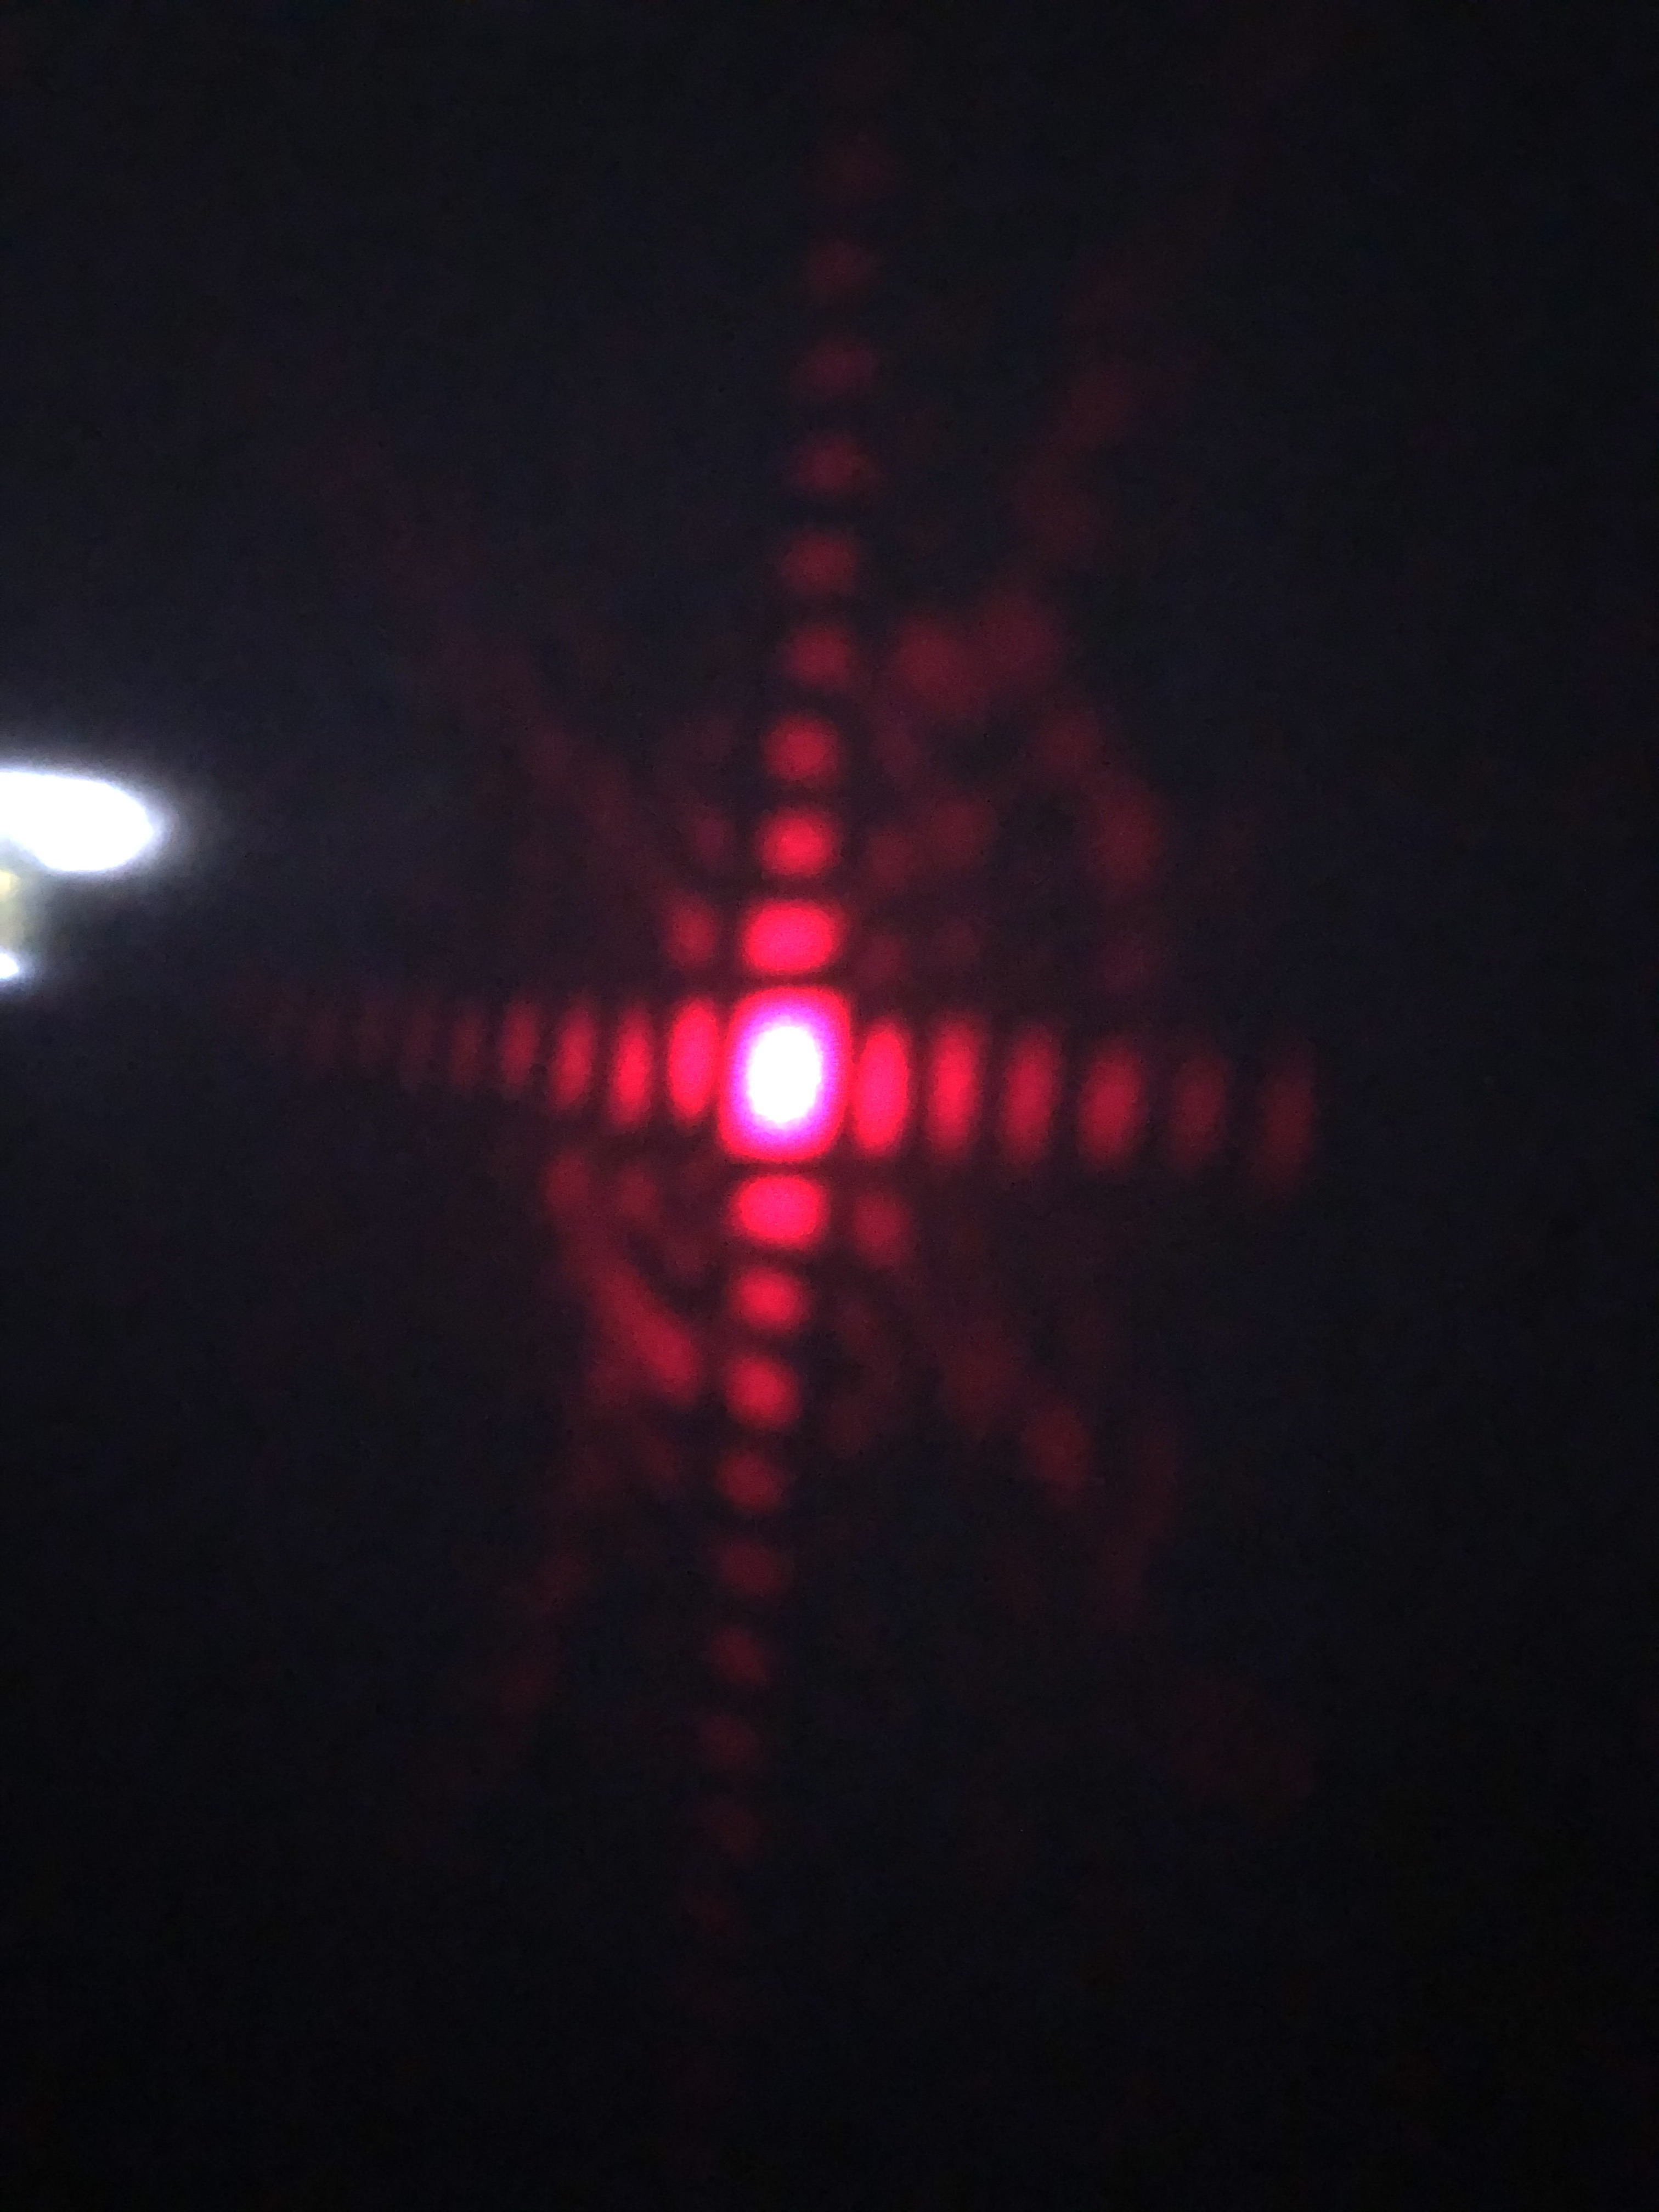
\includegraphics[width = 5cm]{Diffraktion.jpg}
    \end{center}
    \caption{Diffraktionsmönster Rektangulärt hål}
    \label{Rektangel}
\end{figure}

Som visas i figur \ref{Rektangel} fördelades ljuset dels i horisontellt och vertikalt led, men även i diagonaler ut från centrum. Från mönstret tolkas att det rerktangulära hålet är bredare horisontellt än vertikalt eftersom det är glesare mellan huvudmaxima vertikalt och då har ljusets vågfronter böjts starkare i det ledet. I jämförelse med enkelspaltens diffraktionsmönster så utbredde den sig endast i horistontellt led.

\subsubsection{Transmissionsgitter}
En enkel princip för det resulterande mönstret är att varje gitter böjer ljuset och ger upphov till ett interferensmönster med ett antal huvudmaxima. När ljuset passerar ytterligare ett till gitter som böjer ljuset i ett annat led så böjs varje individuellt huvudmaxima ut i det nya ledet så att det  bildas som en matris av huvudmaxima. Om det istället placeras två gitter med samma gitterkonstant som böjer ljuset i samma led, flerdubblas antalet huvudmaxima i det ledet. Det blir då tätare mellan de olika huvudmaxima. 

\begin{figure}[h]
    \begin{center}
        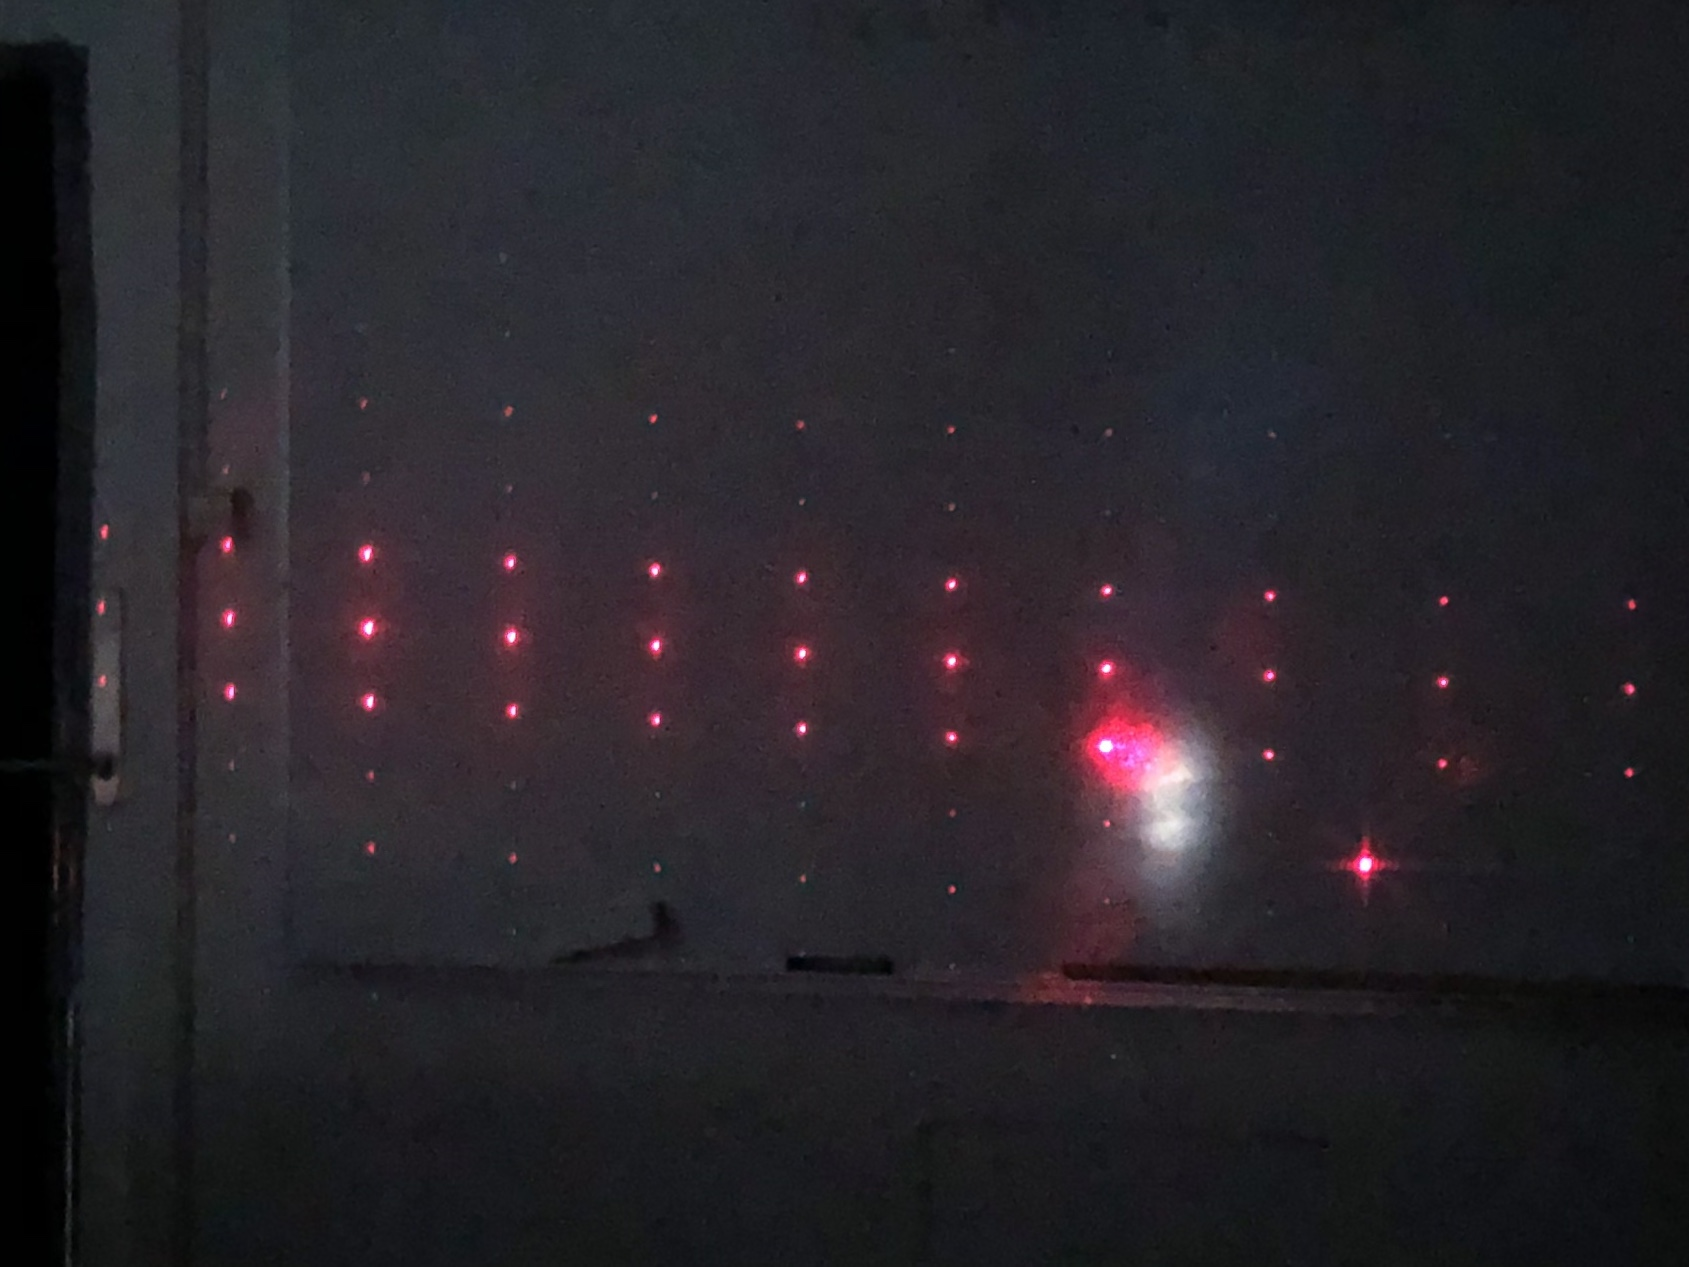
\includegraphics[width = 5cm]{gitter.jpg}
    \end{center}
    \caption{Transmissionsgitter}
    \label{Gitter}
\end{figure}


\subsubsection{Fresneldiffraktion}
Med irisbländaren, när hålet förminskats starkt, böjdes ljuset på ett sätt som gav upphov till destruktiv interferens i mitten av diffraktionsmönstret. Det skulle betyda att om en observation skulle ske från just den punkten i mitten av mönstret, rakt mot laserns öga, skulle det vara mörkt för observatören. 

När det tvärtom var en kula som blockerade vägen för lasern mot väggen så böjdes ljusstrålarna på ett sätt som gav upphov till konstruktiv interferens i mitten av diffraktionsmönstret. Ljuset böjdes alltså runt kulan och träffade väggen. 

\subsection{\textbf{Experiment med gitterspektroskop}}
\emph{Mätresultat första ordningen, (2) är resultat från Hampus grupp:}\vspace{3pt}

\begin{tabular}{|l|r|r|r|} \hline
   \emph{Grader} & \emph{Våglängd(nm)} & \emph{Grader (2)} & \emph{Våglängd(nm) (2)}\\ \hline
    2.65\degree  & 462 & 2.75\degree & 480\\ \hline
    2.70\degree  & 471 & 2.85\degree & 497\\ \hline
    2.85\degree   & 497 & 3.03\degree & 529\\ \hline
    3.65\degree   & 637 & 3.78\degree & 660\\ \hline
    
    \end{tabular} \vspace{5pt}
    
    \emph{Mätresultat fjärde ordningen, (2) är resultat från Hampus grupp:}\vspace{3pt}
    
    \begin{tabular}{|l|r|r|r|} \hline
    \emph{Grader} & \emph{Våglängd(nm)} & \emph{Grader (2)}& \emph{Våglängd(nm) (2)}\\ \hline
    10.75\degree  & 466 & 10.88\degree & 472\\ \hline
    11.08\degree  & 480 & 11.12\degree & 482\\ \hline
    11.72\degree  & 508 & 11.78\degree & 511\\ \hline
    15.00\degree     & 647 & 14.95\degree & 645\\ \hline
    
    
\end{tabular} \vspace{5pt}

Våglängdsavvikelsen till de verkliga värdena är lägre vid fjärde ordningen eftersom mätningen av vinkeln betyder mindre desto längre ut från centrum. Detta kommer ur gitterformeln, se \cite{Handledningen}. Atomslaget som bäst matchar dessa mätresultat är [Cd]kadmium. 

\subsection{\textbf{Diffraktion i N spalter}}
\begin{tabular}{|l|c|r|} \hline
\emph{Antal spalter} & \emph{Spaltbredd($\mu$m)}  & \emph{Spaltavstånd}\\ \hline
1 & 50 & NA\\ \hline
2 & 45 & 100\\ \hline
3 & 48 & 100\\ \hline
4 & 45 & 100\\ \hline
\end{tabular} \vspace{5pt}

\begin{figure}[H]
    \begin{center}
        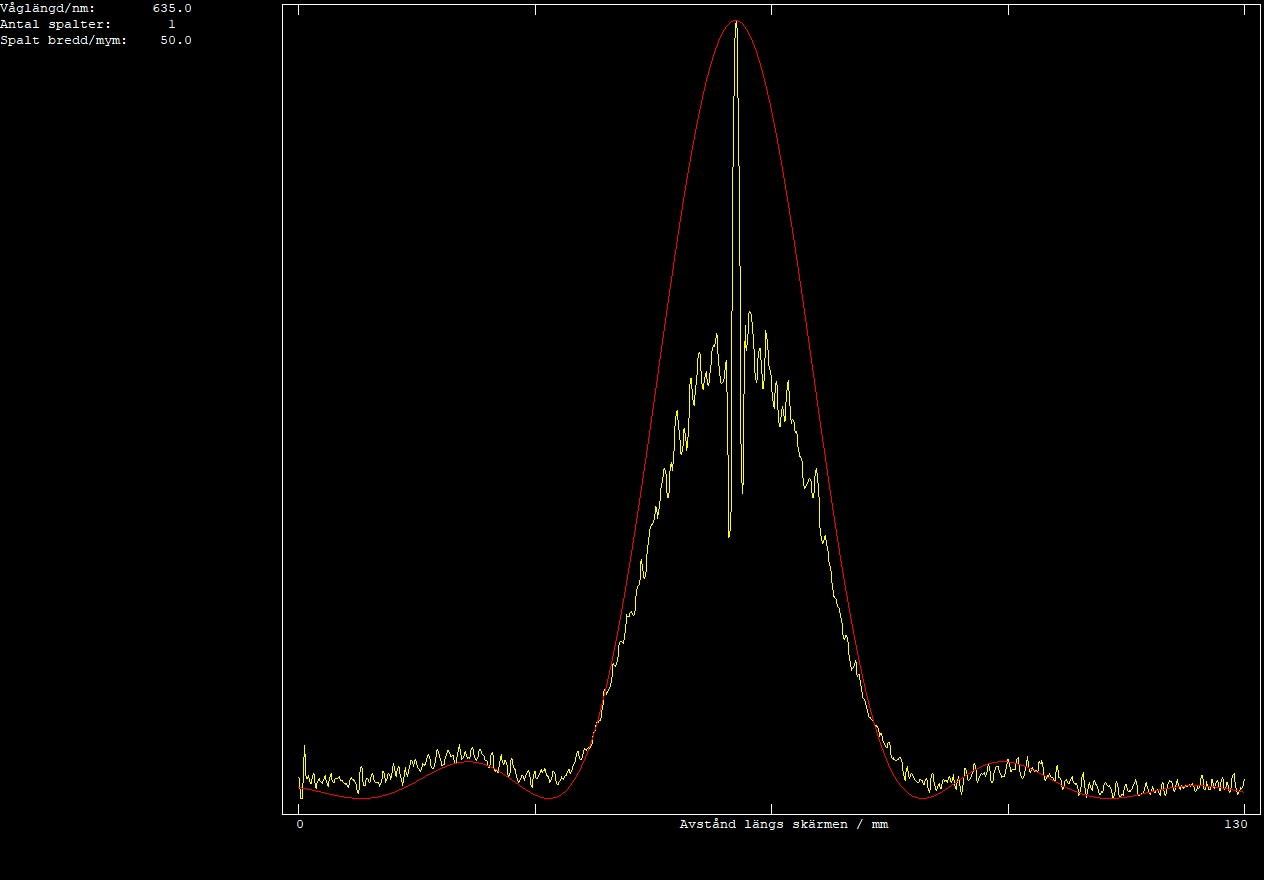
\includegraphics[width = 8 cm]{first.jpg}
    \end{center}
    \caption{En spalt, x: Avstånd längs skärmen(mm), y: Ljusintensitet}
    \label{1 spalt}
\end{figure} \vspace{3pt}

\begin{figure}[H]
    \begin{center}
        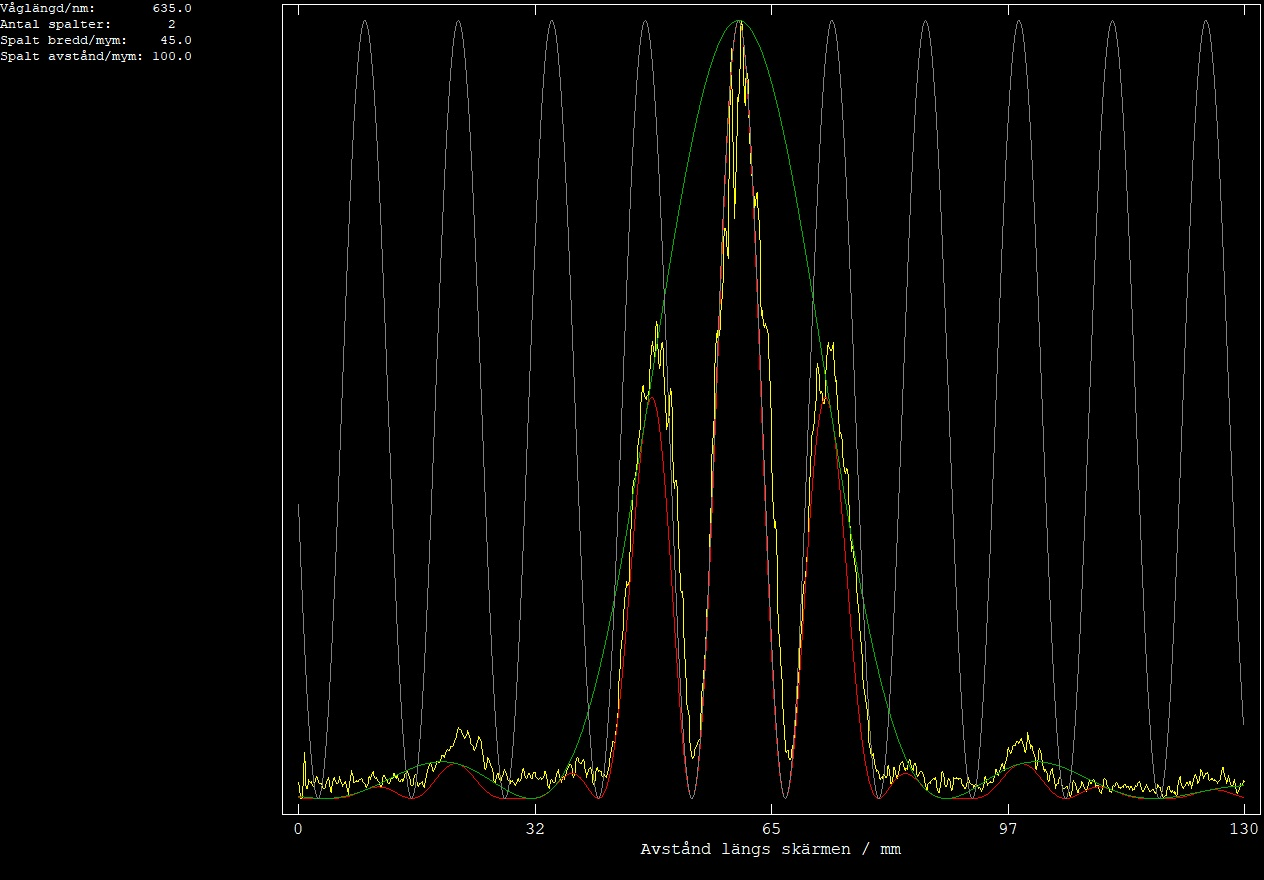
\includegraphics[width = 8cm]{Andra.jpg}
    \end{center}
    \caption{Två spalter, x: Avstånd längs skärmen(mm), y: Ljusintensitet}
    \label{2 spalter}
\end{figure} \vspace{3pt}

\begin{figure}[H]
    \begin{center}
        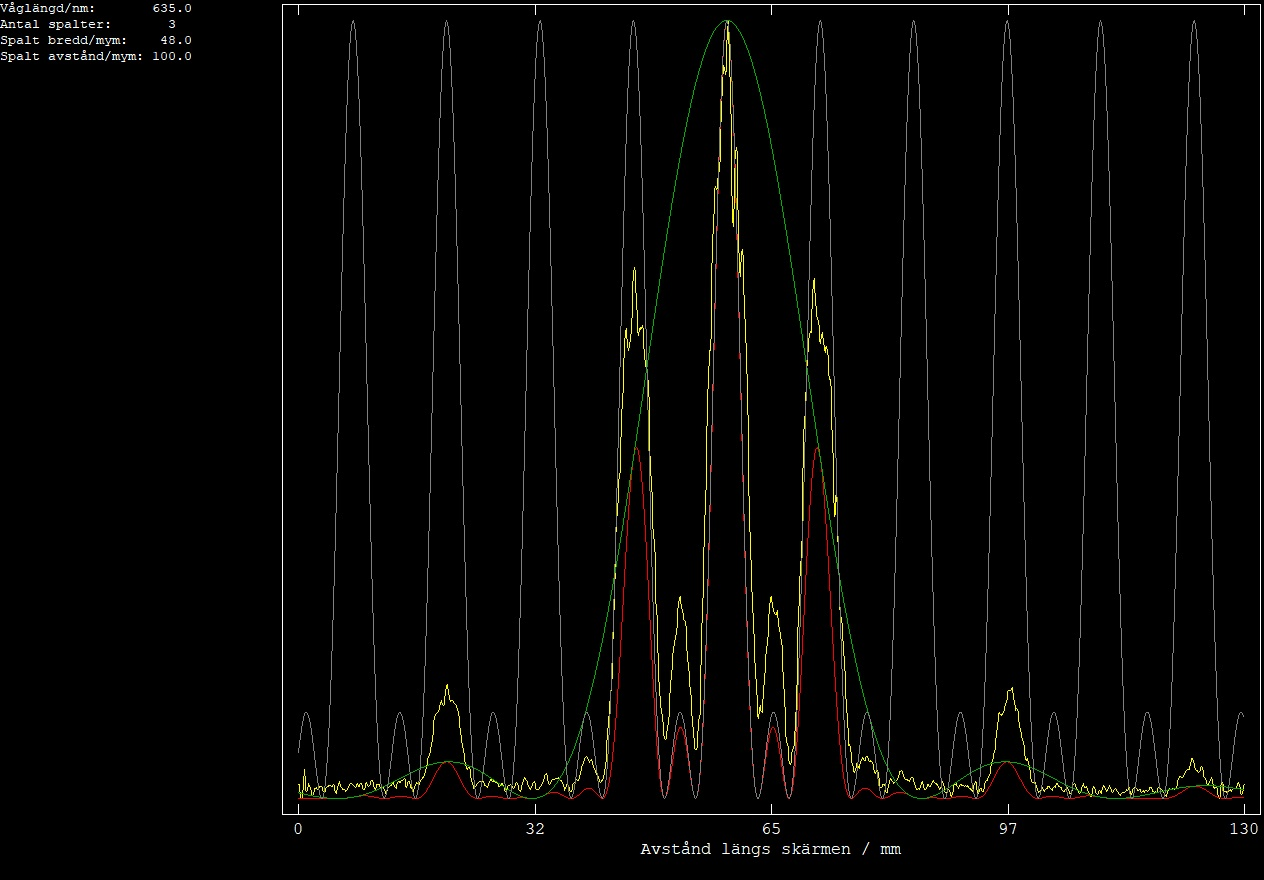
\includegraphics[width = 8cm]{Tredje.jpg}
    \end{center}
    \caption{Tre spalter, x: Avstånd längs skärmen(mm), y: Ljusintensitet}
    \label{3 spalter}
\end{figure} \vspace{3pt}

\begin{figure}[H]
    \begin{center}
        \includegraphics[width =8cm]{Fjärde.jpg}
    \end{center}
    \caption{Fyra spalter, x: Avstånd längs skärmen(mm), y: Ljusintensitet}
    \label{4 spalter}
\end{figure} \vspace{3pt}

\begin{figure}[H]
    \begin{center}
        \includegraphics[width = 8cm]{Grön.jpg}
    \end{center}
    \caption{Grön laser okänd våglängd, x: Avstånd längs skärmen(mm), y: Ljusintensitet}
    \label{Grön laser}
\end{figure} \vspace{3pt}
Den gröna laserns våglängd uppmättes av Jacob \& Richards grupp samt Hampus grupp till 520 nm respektive 530nm. 

%-------------------------------------------------------------------------

\section{Diskussion}

\subsection{Diffraktionsexperiment med laserljus}
Med formeln för böjningsminimum för en spalt och ett hål, given information om ljuset och beräkning av vinkeln kunde spaltbredden på enkelspalten och det cirkulära hålet bestämmas. Det relativt precisa resultatet kan troligtvis tillskrivas att beräkningarna av vinkeln gjordes på ett intensitetsminima av hög grad och att avståndet mellan ljuskällan och väggen som diffraktionsmönstret avbildades på var stort; därmed blev mätfelen för mätningarna av sträckorna relativt små. 

Att det bildas diffraktionsmönster både i x- och y-led, som figur 1 visar, för det rektangulära hålet till skillnad från en vanlig spalt som endast får ett tydligt diffraktionsmönster på ena ledden kan även beskrivas av fraunhoferdiffraktion. Till skillnad från en vanlig spalt har det rektangulära hålet både en begränsad höjd och bredd vilket leder till att ljuset böjs i båda ledderna. Från experimentet går det att avläsa att hålet är horisontellt rektangulärt (mindre höjd än bredd) då diffraktionsmönstret var mer utdraget i den vertikala ledet än vad det var i det horisontella ledet, vilket ligger i linje med att ljuset böjs mer ju smalare öppningen är. 

Det diffraktionsmönster som uppstod då ljuset gick igenom ett gitter består av en mängd nästintill identiska ljusmaxima med identiska minimum mellan. Alltså går det inte att urskilja ett centralmaximum och vilken grad övriga maximum är av som det går då ljuset böjs i en eller några enstaka spalter. Detta beror på att varje spaltöppning i gittret skapar en egen vågfront; när alla interfererar bildas ett jämnt mönster där varje maximum har ungefär samma storlek på grund av att varje maximum är en produkt av positiv interferens mellan liknande vågfronter; däremot minskar intensiteten för maximumen ju längre från centrum man undersöker då maximumen är ett resultat av att färre vågor interfererar. 

Att kombinera två gitter, en med spalterna vertikalt och en med spalterna horisontellt, resulterade i ett liknande diffraktionsmönster fast i ett helt plan. Detta beror på att varje punkt i det diffraktionsmönster som bildas av det första gittret sedan böjs i det andra gittret som är positionerat på den andra ledden och därmed bildar ett diffraktionsmönster av diffraktionsmönstret; alltså sprids mönstret längs båda axlarna. 

När irisbländarens öppning justerades bildades ett hål i mitten av ljuset, stort ungefär som öppningen. Detta kan förklaras med fresneldiffraktion.  När den cirkulära skivan med en kula i mitten användes inträffade det motsatta; i mitten av ljusmönstret på väggen blev det ett maximum med ett ringformat minimum runt om. Detta beror också på fresneldiffraktion. Runt om, alltså motsvarande öppningen i skivan, blir det en ring av negativ interferens och därmed intensitetsminimum. 



\subsection{Experiment med gitterspektroskop}
Jämfört med andra experiment som mätt våglängderna för spektrallinjer hos kadmium-ljus, avviker de uppmätta våglängderna i fjärde ordningen i denna laboration endast med några enstaka nanometer \cite{NIST}. Jämfört med NIST var våglängderna som uppmättes i denna laboration 1,8nm (0,38\%) lägre för den mörkblå spektrallinjen, 0,6nm (0,12\%) lägre för den gröna spektrallinjen och 0,5nm (0,08\%) högre för den röda spektrallinjen \cite{NIST}. De våglängder som mättes i första ordningen avvek avsevärt mer från de riktiga våglängderna än de som mättes i fjärde ordningen (för båda laborationsgrupper), vilket visar att mätningarna blir mer precisa desto högre ordning som mäts. Detta kan bero på att avståndet mellan de olika spektrallinjerna i en låg ordning är liten, vilket gör att vinkeln måste vara mer precis om avståndsförhållandet mellan två spektrallinjer ska stämma. En felmätning på exempelvis 0,1\degree har mycket större påverkan på en liten vinkel (tex. 3\degree) än det har på en större vinkel (tex. 15\degree); vinkeln blir 3,3\% respektive 0,7\% fel. 

Resultaten från den ena laborationsgruppen låg alltid under den verkliga våglängden, medan resultaten från den andra gruppen låg över i den första ordningens mätningar. Vad detta beror på är svårt att klargöra, men oerfarenhet av mätningar med nonieskala hos en eller båda grupper är en möjlig anledning. Dessa skillnader stämde även för den fjärde ordningen även om felmarginalen minskades betydligt, vilket tyder på att båda grupper var konsekventa i sina mätningar. Om den roterande plattan på gitterspektroskopet haft en större diameter, hade fler rister fått plats längs plattans kant, så att vinkeln kunnat mätas mer exakt. 

Efter att de uppmätta våglängderna för ljuset i spektroskopet jämfördes med en tabell kunde det konstateras att lampan innehöll kadmium-atomer. Tabellen visade att kadmium emitterar fotoner med våglängder som matchade alla de våglängder som räknades ut i laborationen. 

\subsection{Diffraktion i N spalter}
Enligt teorin är antalet minimum mellan två huvudmaxima ett lägre än antalet spalter i systemet. Ur figurer 3 till 7 blev det därför tydligt att de olika spaltsystemen hade 1, 2, 3 eller 4 spalter. Enligt uträkning i handledningen blir topparna smalare och skillnaden mellan huvuvmax och bimax större ju fler spalter ljuset går igenom \cite{Handledningen}, vilket också kunde avläsas tydligt i intensitetsdiagrammen. I en jämförelse mellan figur fem och sex, syns det att bimax I figur sex är ungefär hälften så höga som i figur fem. 

Det syns att spaltbredden är lika stor hos de olika spaltsystemen eftersom den gröna kurvan, enkelspaltfaktorn, har samma kurva i figurer tre till sex (och sju). 

Med hjälp av datorprogrammet kunde den ungefärliga våglängden för det gröna ljuset estimeras. Jacob \& Richards grupp samt Hampus grupp kom fram till att det gröna ljuset var 520nm respektive 530nm. Den korrekta våglängden för ljuset var 532nm, vilket var relativt nära. Feluppskattning kan bero på ett antal faktorer; fel avstånd mellan spalt och skärm, hur stor del av skärmen som kameran fotograferade, spaltbredd och spaltavstånd. Alla dessa faktorer påverkar datorprogrammets analys. 
\begin{comment}
Om uträkningarna gjorts för hand hade vinkeln $\theta = \arctan(\frac{4,9~\text{cm}}{2,02~\text{m}})$ = 1.39\degree. Enligt formeln för huvudmaximum hade detta gett våglängden $\lambda = \frac{45\mu m \times \sin(1,39\degree)}{3} = 364 nm$. Detta eftersom avståndet till tredje huvudmaxima uppmättes till 4,9 cm och avståndet mellan spalterna och skärmen var 2,02 m. Detta är dock mycket lägre än den korrekta våglängden hos den gröna lasern. En möjlig anledning till denna stora felmarginal är att denna beräkning gjordes på mätdata för ett maxima av låg ordning (tredje). Om ordningen är låg blir felmarginalen större, av samma anledning som beskrevs i diskussionen om gitterspektroskopet. Felet är dock ändå stort även med denna felmarginal, så det är mycket möjligt att ett mätfel har uppstått - exempelvis att fel huvudmax har avlästs, eller att det var ett bimax som lästes av istället för ett huvudmax. 
\end{comment}

Med bättre utrustning (starkare laserljus, känsligare kamera etc.) desto tydligare hade kurvuorna i resultaten blivit, så att det blivit lättare för det blotta ögat att att se olika bimax, huvudmax och interferensminimum. Däremot var utrustningen lagom för att datorn skulle kunna bestämma våglängden med bra precision. 




%-------------------------------------------------------------------------

\section{Sammanfattning}

I första delen av laborationen beräknades spaltbredden i enkelspalten och diametern av det cirkulära hålet till 0,25 mm m.h.a. mätningar i diffraktionsmönstret. Fraunhoferdiffraktion i en rektangulär öppning och i ett gitter studerades kvalitativt och jämfördes med fresneldiffraktion. Det observerades att fresneldiffraktion medförde att det är möjligt att titta rakt in i en ljuskälla, utan att se något ljus, och att det även är möjligt att titta på ett objekt som är placerat mitt framför en ljuskälla, men ändå se ljuset. Detta går emot intuitionen, men kan förklaras av konstruktiv och destruktiv interferens då ljusvågorna från ljuskällan böjs hos objektet framför eller runtom ljuset. 

I andra delen av laborationen mättes vinklar för spektrallinjer i olika ordningar i ett gitterspektroskop. När vinklarna mätts kunde våglängderna för ljuset beräknas, och ur resultatet kunde det konstateras att mätningarna blev mer precisa desto högre ordning som mättes. Detta stämde för två olika gruppers mätdata, även om den första gruppens mätvärden i den första ordningen gav lite för korta våglängder och den andra gruppens mätvärden gav lite för långa våglängder. Genom att matcha gruppens uppmätta våglängder med en tabell med emissionsvåglängder för olika atomslag syntes det att lampan i gitterspektroskopet innehöll kadmium-atomer. 

I den tredje delen av laborationen mättes diffraktionsmönstret då en röd laser användes på fyra olika gitter och därefter även en grön laser på det ena gittret. Ett datorprogram genererade diagram över diffraktionsmönstrenas intensitetsfördelning som antalet spalter, spalternas bredd och deras avstånd från varandra för de fyra gitterna kunde avläsas från. Därefter bestämdes våglängden på den gröna lasern med ett sådant datorgenererat diagram. Datorprogrammet bestämde med hög precision våglängden.

%-------------------------------------------------------------------------











%Om man har referenserna i en databas, i det här fallet filen references.bib
%\bibliographystyle{plain}
%\bibliography{../../references} 

%Alternativt om man skriver referenserna direkt här i filen

\begin{thebibliography}{77}
	
\bibitem{Fraunhofer}G. Jönsson: \emph{Våglära och Optik}, 5:e upplagan, Lund Sverige: Teach Support

\bibitem {Handledningen}Labbhandledningen: \emph{Ljusets Diffraktion}, 2020

\bibitem{NIST}National Institute of Standards and Technology: \emph{Basic Atomic Spectroscopic Data}, Accessed on: 2020.03.04, Available: https://physics.nist.gov/PhysRefData/Handbook/Tables/cadmiumtable2_a.htm

\end{thebibliography}

\end{document}